\documentclass[12pt]{article}
\usepackage[brazilian]{babel}
\usepackage[utf8]{inputenc}
\usepackage{setspace}
\usepackage{boxedminipage}
\usepackage{amsmath}
\usepackage{latexsym}
\usepackage{multirow}
\usepackage[pdftex]{graphicx}
\usepackage{float}
\usepackage{url}
\usepackage{tikz}
\usetikzlibrary{bayesnet}
\usepackage{blkarray}

\renewcommand{\familydefault}{\sfdefault}
\newcommand{\question}[2] {\vspace{0.3in}\noindent{\subsection*{Exercício #1. #2} \vspace{0.15in}}}
\renewcommand{\part}[1] {{\vspace{0.15in}\noindent\textbf (#1)} \vspace{0.10in}}
\newcommand{\answer}[1]{{\fontfamily{\rmdefault}\selectfont \textbf{R:} #1}}
\newcommand{\overbar}[1]{\mkern 2mu\overline{\mkern-2mu#1\mkern-2mu}\mkern 2mu}

%\setlength{\parskip}{0.1cm}
\setlength{\paperheight}{29.7cm}
\setlength{\textheight}{23.0cm}
\setlength{\textwidth}{16.5cm}
\setlength{\oddsidemargin}{0.0cm}
\setlength{\topmargin}{-1.0cm}
\pagestyle{empty}


\begin{document}
\title{Lista de exercícios de Introdução à Redes Booleanas Probabilisticas}
\author{\large Gustavo Estrela de Matos}
\date{\today}
\maketitle

\question{9}{Reproduza os resultados do paper "Generating 
Boolean networks with a prescribed attractor structure".}

\begin{figure}[H]
  \centering
  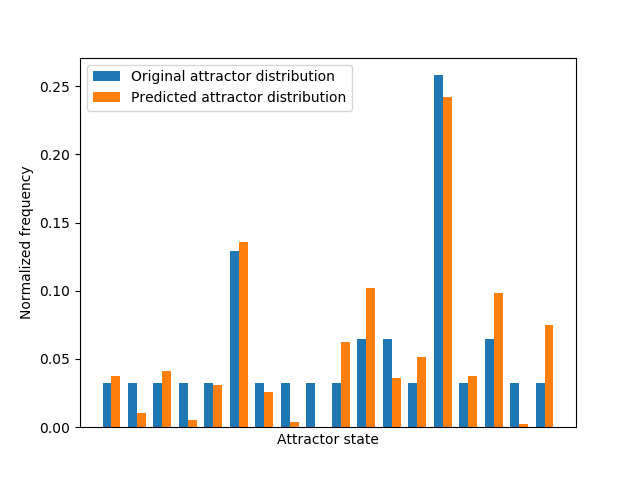
\includegraphics[width=.7\textwidth]{results.png}
\end{figure}
\end{document}

